\documentclass[tikz,border=5pt]{standalone}
\usetikzlibrary{3d,calc,positioning}
\begin{document}

% User‐controllable parameters:
\def\Nu{20}    % number of subdivisions in u‐direction
\def\Nv{20}    % number of subdivisions in v‐direction
\def\ArrStep{2} % step for vector‐field sampling (in grid units)

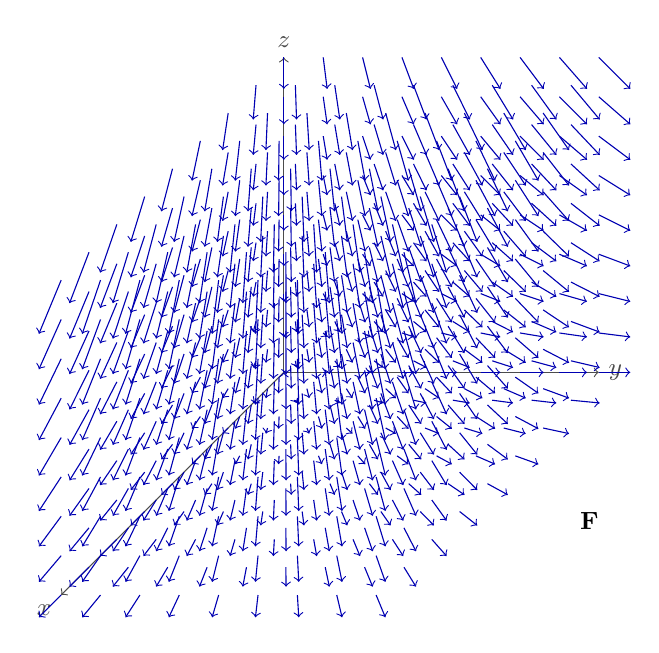
\begin{tikzpicture}[
	% 3D projection:
	x={(-0.707cm,-0.707cm)},  % x→SW
	y={(1cm,0cm)},            % y→E
	z={(0cm,1cm)},            % z→N
	font=\small,
	axis/.style={->,black!70},
	grid/.style={gray!30,very thin},
	surf/.style={red!50},
	surflight/.style={red!20},
	vf/.style={->,blue!70!black},
	scale=2
	]
	
	%
	% Panel 1: (u,v) domain
	%
	\begin{scope}[shift={(-5cm,0)}]
	% Axes 0→3
	\draw[axis] (0,0,0)--(2,0,0) node[anchor=north east]{$x$};
	\draw[axis] (0,0,0)--(0,2,0) node[anchor=west]{$y$};
	\draw[axis] (0,0,0)--(0,0,2) node[anchor=south]{$z$};
	
	% full field on [0,3]^3 integer grid
	\foreach \x in {0,.25,.5,...,2}{
		\foreach \y in {0,.25,.5,...,2}{
			\foreach \z in {0,.25,.5,...,2}{
				\draw[vf] (\x,\y,\z) -- ++(0.1*\x,0.1*\y,0.1*-\z);
			}
		}
	}
	\node[above] at (1.5,3,0) {$\mathbf F$};
	\end{scope}
	%
	% Panel 2: Parametric surface mesh
	%
%	\begin{scope}[shift={(0,0)}]
%		% axes
%		\draw[axis] (0,0,0)--(2,0,0) node[anchor=north east]{$x$};
%		\draw[axis] (0,0,0)--(0,2,0) node[anchor=west]{$y$};
%		\draw[axis] (0,0,0)--(0,0,2) node[anchor=south]{$z$};
%		% mesh lines u=const
%		\foreach \i in {0,...,\Nu} {
%			\pgfmathsetmacro\u{\i/\Nu}
%			\draw[surf] plot[domain=0:1,variable=\v]
%			({\u+2*\v},{2*\u+\v},{3*\u*\v});
%		}
%		% mesh lines v=const
%		\foreach \j in {0,...,\Nv} {
%			\pgfmathsetmacro\v{\j/\Nv}
%			\draw[surf] plot[domain=0:1,variable=\u]
%			({\u+2*\v},{2*\u+\v},{3*\u*\v});
%		}
%		\node[above] at (1.5,3,0) {Surface $\mathbf r(u,v)$};
%	\end{scope}
	
	%
	% Panel 3: Surface + vector field
	%
%	\begin{scope}[shift={(5cm,0)}]
%		% axes
%		\draw[axis] (0,0,0)--(2,0,0) node[anchor=north east]{$x$};
%		\draw[axis] (0,0,0)--(0,2,0) node[anchor=west]{$y$};
%		\draw[axis] (0,0,0)--(0,0,2) node[anchor=south]{$z$};
%		% light mesh
%		\foreach \i in {0,...,\Nu} {
%			\pgfmathsetmacro\u{\i/\Nu}
%			\draw[surflight] plot[domain=0:1,variable=\v]
%			({\u+2*\v},{2*\u+\v},{3*\u*\v});
%		}
%		\foreach \j in {0,...,\Nv} {
%			\pgfmathsetmacro\v{\j/\Nv}
%			\draw[surflight] plot[domain=0:1,variable=\u]
%			({\u+2*\v},{2*\u+\v},{3*\u*\v});
%		}
%		% vector‐field arrows
%		\foreach \i in {0,\ArrStep,...,\Nu} {
%			\foreach \j in {0,\ArrStep,...,\Nv} {
%				\pgfmathsetmacro\u{\i/\Nu}
%				\pgfmathsetmacro\v{\j/\Nv}
%				\pgfmathsetmacro\x{\u+2*\v}
%				\pgfmathsetmacro\y{2*\u+\v}
%				\pgfmathsetmacro\z{3*\u*\v}
%				\pgfmathsetmacro\Fx{\x}
%				\pgfmathsetmacro\Fy{\y}
%				\pgfmathsetmacro\Fz{-\z}
%				\draw[vf] (\x,\y,\z) -- ++(0.15*\Fx,0.15*\Fy,0.15*\Fz);
%			}
%		}
%		\node[above] at (1.5,3,0) {Surface and $\mathbf F$};
%	\end{scope}
\end{tikzpicture}
\end{document}
